\begin{figure}[htp]
\centering
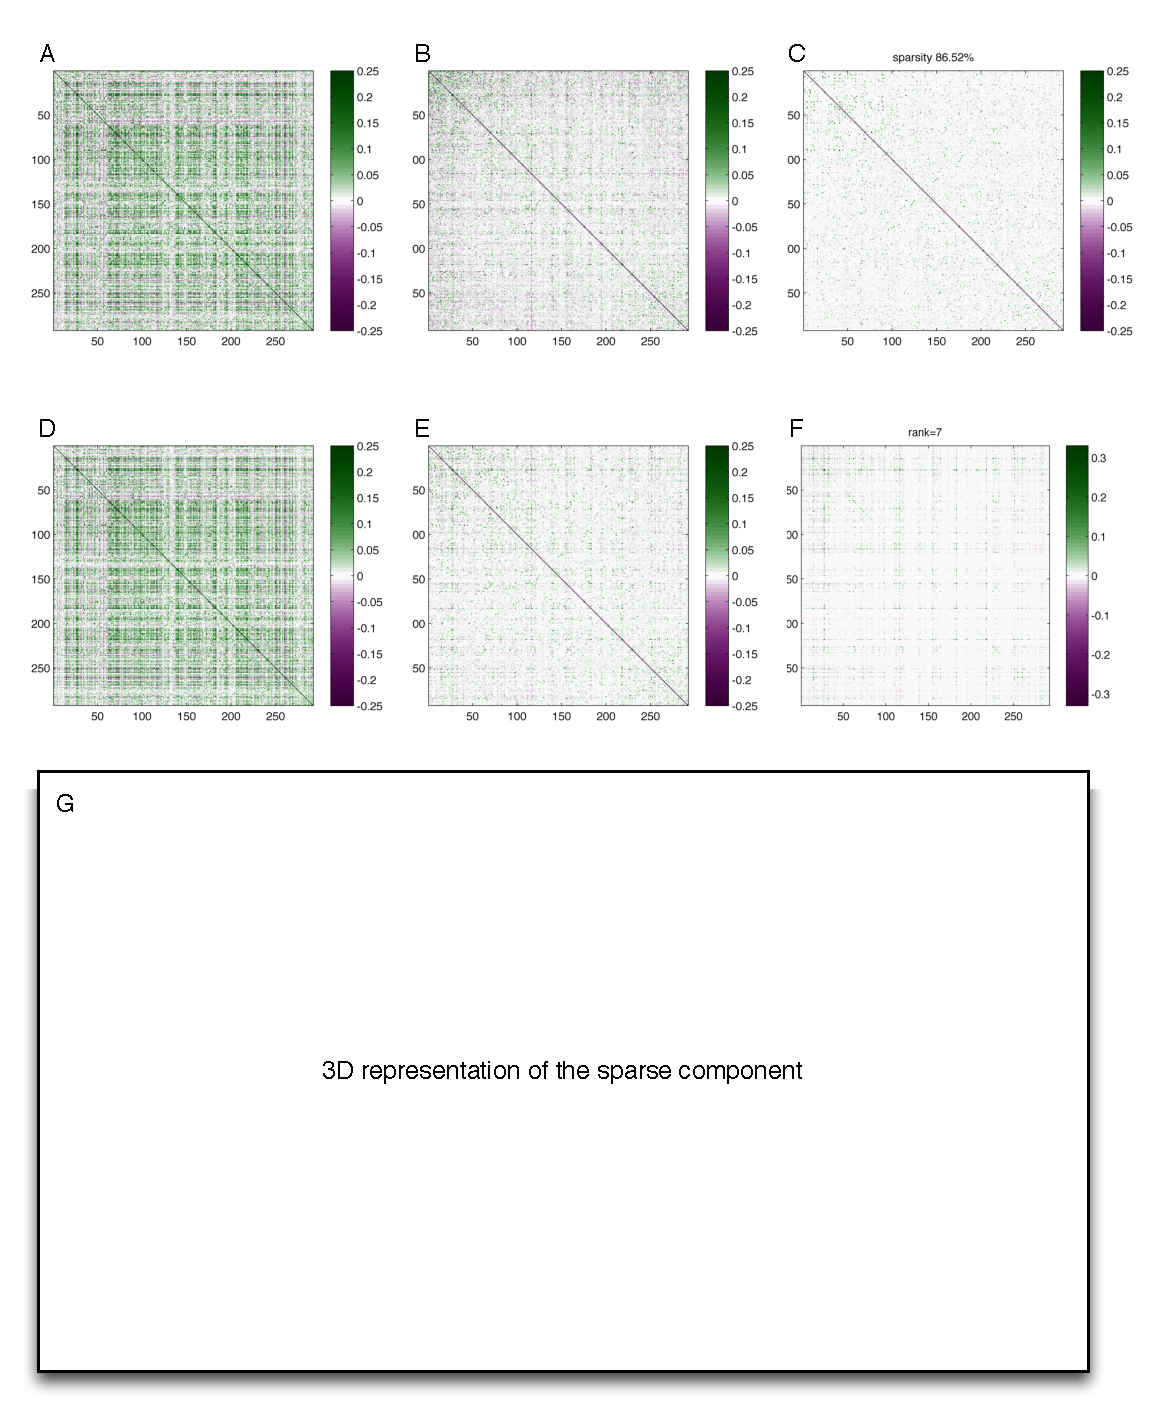
\includegraphics[width=0.5\textwidth]{figures/Figure5.pdf}
\caption{
Example of covariance structure revealed by the sparse+low-rank estimator and its relationship to the circuit arcitecture.
{\bf A:} The correlation matrix from Fig.~\ref{fig:01}D. 
{\bf B:} Partial pairwise correlations (scaled negative inverse of the correlation matrix in {\bf A}) 
{\bf C:} Optimal cross-validated sparse+latent estimate of the corrleation matrix from the same dataset. 
{\bf D:} Negative inverse of the sparse+latent estimate in {\bf C}. 
{\bf E:} The sparse component of {\bf D} with 96.5\% off-diagonal coefficients set to zero with the average of 5.1 edges per cell.
{\bf F:} The low-rank component of {\bf D}, rank=7.
{\bf G:} The spatial arrangement of cells used in the analysis, connected by edges that correspond to the non-zero elements of the sparse component in {\bf E}. Green edges denote positive weights, red edges denote negative weights.  Color-filled cells are significantly tuned to grating orientation as indicated by the color code in the legend.
}
\label{fig:05}
\end{figure}
